% !TEX root = ../notes_template.tex
\chapter{Oral Microbiome}\label{chp:oral_microbiome}

\minitoc

\section{Introduction}
\epigraph{\emph{I didn't clean my teeth for three days and then took the material that had lodged in small amounts on 
the gums above my front teeth… I found a few living animalcules}}{- Antonie van Leeuwenhoek's letter to the Royal Society 
on observations made from his own dental plaque, translated by Clifford Dobell}

Despite being considered by many as a relatively modern field of research, the first descriptions of human-associated 
microbiota date back to the 1670s-1680s, when Antonie van Leeuwenhoek started using his newly developed, handcrafted microscopes. 
In a letter written to the Royal Society of London in 1683, he described and illustrated five different kinds of bacteria 
(although he called them animalcules at the time) present in his own mouth and that of others, and subsequently also 
compared his own oral and faecal microbiota, determining that there are differences between body sites as well as between 
health and disease. Some of the first direct observations of bacteria were of human-associated microbiota.


The oral microbiome is the second large microbiome in the human body, after the gut, with more easy access. Presents spatially organized 
biofilms \cite{Welch2020,Wilbert2020}, which derives in the site-specialist hypothesis that predicts that most microbes 
in the human oral cavity have a primary \gls{habitat} type within the mouth where they are most abundant. 

Importance of the spatial organization in various aspects of the human microbial ecology \cite{Proctor2017}.

Studies have revelead that the microbes living in the oral cavity are a major contributor to the overall host health 
\cite{Hajishengallis2021}. In periodontal disease, there is a low-grade systemic inflammatory state
\footnote{gls{low-grade systemic inflammation}}
that has been mechanistically linked to multiple chronic inflammatory diseases such as \acrfull{t2dm}
and \acrfull{cvd}. The host immune response is tightly intertwined with metabolism,
and dysfunction of this integrated system may lead to chronic metabolic inflammatory disorders.

\section{Previous studies}
Most of the oral microbiome research has been based on 16S rRNA gene amplicon sequencing studies \cite{Escapa2018}
Metagenomic studies:
\begin{itemize}
    \item \citetitle{Zhu2022}. Includes:
    \begin{itemize}
        \item 
    \end{itemize}
\end{itemize}

\section{Major oral habitats}
The mouth is an open system. Microbes are breathed with the air, ingested with the food, or acquired through close 
contact (animals, humans, or surroundings). 

Although the millions of bacterial species on the planet discovered so far (and other millions to remain discovered), 
it is believed that only approximately 760\footnote{In my opinion this number is not informative, as don't 
take into account any prevalance among population, including rare and probably transient species} are primary residents, rather than transients in the mouth, according to the 
Human Oral Microbiome Database \cite{Escapa2018} .
\begin{itemize}
    \item Supragingival plaque
    \item Subgingival plaque 
    \item Keratinized gingiva 
    \item Hard palate 
    \item Buccal mucosa 
    \item Throat 
    \item Palatine tonsils 
    \item Tongue dorsum 
\end{itemize}

Each of these sites is not monolithic, rather sheltered or exposed to different environmental conditions: 
\begin{itemize}
    \item Crowns of teeth abundant of oxygen.
    \item Tooth surface in the gingival crevice anorexic environment bathed in gingival crevicular fluid, protein-rich 
    exudate from the gingival tissues. 
    \item Saliva film thinnest at the roof of the mouth in contrast with the saliva pools at the floor. 
    \item Similarly, relative proximity to salivary glands influences the composition and rate of flow of saliva. 
\end{itemize}

Although saliva is not a habitat per se, there are evidence that microbes found within the saliva are not abundant at 
any of the other sampled sites, suggesting additional unique micro-habitats elsewhere in the mouth. 

\section{Selective force within the mouth}
Flow and adhesion
\begin{itemize}
    \item Salivary flow imposes a selective requirement for adherence: microbes can persist in exposed locations in the 
    mouth only if they are adhered to an underlying substrate or to other microbes that are able to adhere to the substrate. 
    \item In addition, salivary flow also requires closely proximity for microbial interactions, as microbial metabolites 
    are constantly washed. Interestingly,  
    \item In response to selective pressures, oral microbes developed highly specific adhesin-receptor interactions, 
    which form the basis for cohesion or coaggregation phenomenon. 
\end{itemize}
Shedding and colonization
\begin{itemize}
    \item Dynamics of shedding of the underlying substrate and re-colonization back to the substrate.
    \item Overall thickness of the microbial biofilm is influenced by the rate of shedding. Exposed areas: enamel teeth 
    surface, mucosal surfaces. Factors: oral hygiene, abrasion by chewing food. 
    \item Colonization of fresh substates after shedding and abrasion. This colonization is dependent on both microbial 
    and host sources, e.g. colonizing streptococci bind to cysteine repeat domains within glycoproteins or sialic acid of 
    mucin in the enamel pellicle, whereas adherence of specific bacteria to the mucosa could be mediated in part by the secretory 
    immunoglobulin A.
\end{itemize}
Host and microbe
\begin{itemize}
    \item Saliva flow and immune surveillance are properties of the host that reduce the microbial load. 
    \item Saliva is also a vehicle for positive selection of microbes cause mucins and nutrients such as lactate, 
    bicarbonate, nitrate, and vitamins are actively secreted into saliva \cite{Carpenter2020}.
\end{itemize}

Testing figs (\autoref{fig:saliva_content},\autoref{fig:urea_test})

\begin{figure}[!ht]
    \centering
    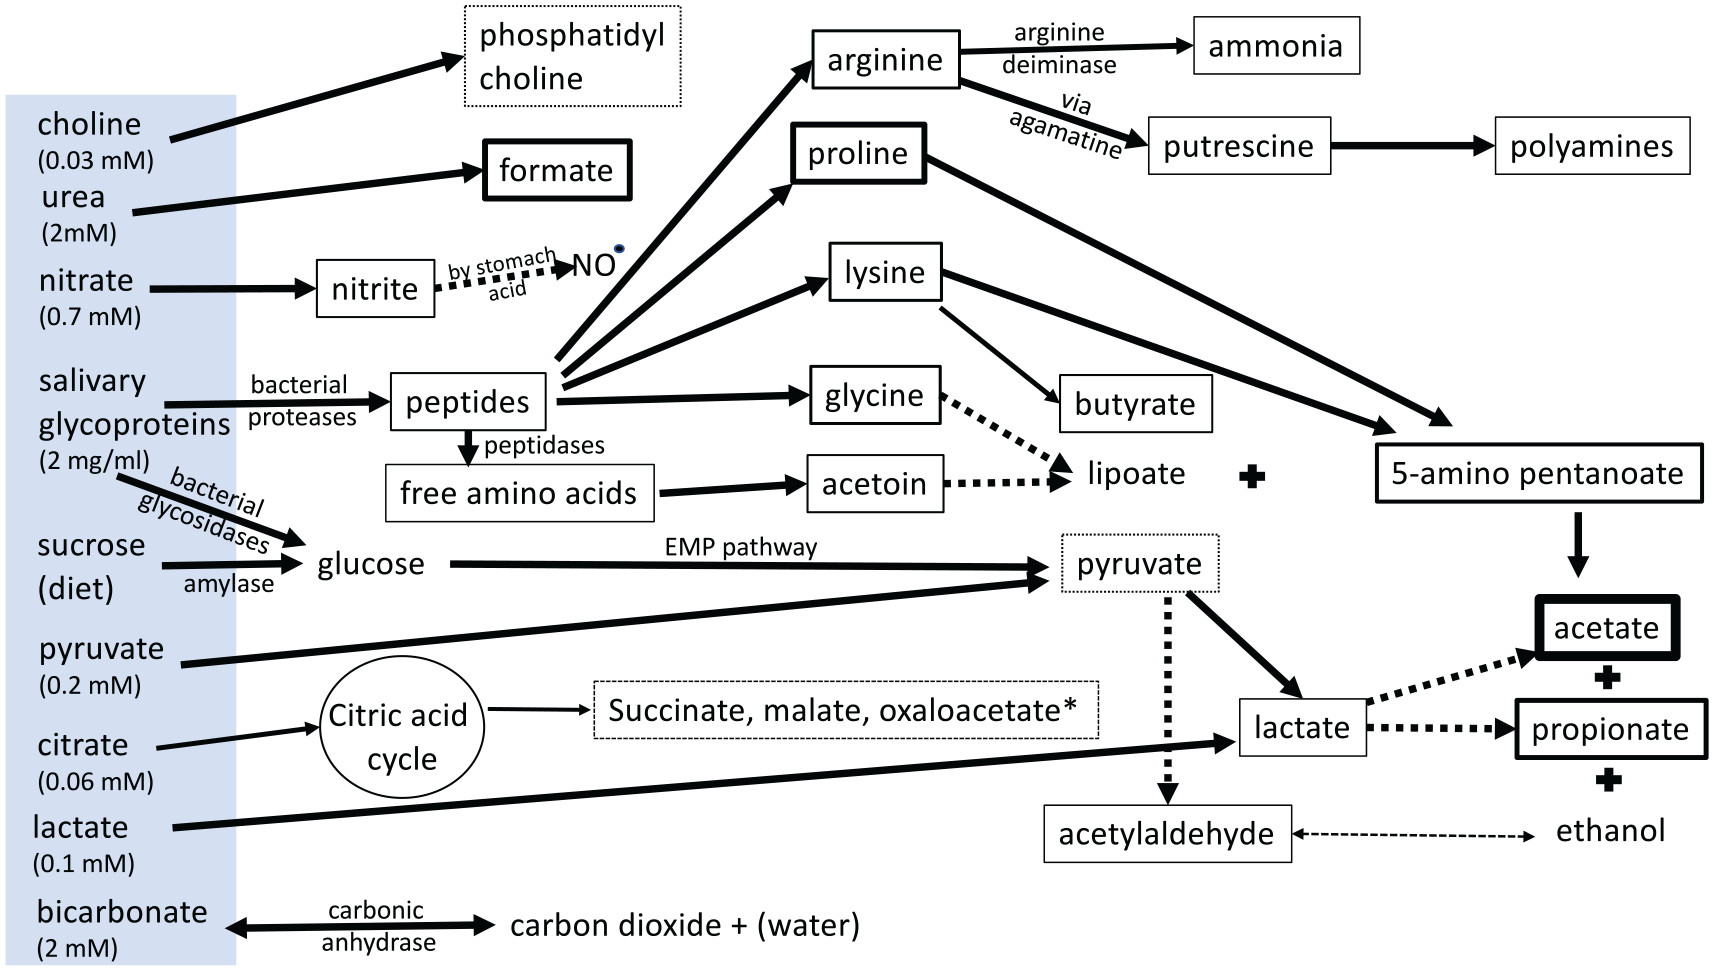
\includegraphics[width=1\linewidth]{./figure/saliva_content.jpeg}
    \caption{The main bacterial substrates (blue box) and detected metabolites (indicated by boxes) in whole mouth saliva. 
    The thickness of arrows and boxes indicates relative abundance, dotted lines indicate possible connections. 
    Under resting conditions between meals, the products of the citric acid cycle (indicated by *) are largely undetectable. 
    Most metabolites indicate the breakdown of salivary glycoproteins as the main nutrient source, the amino acids 
    yielding acetate and propionate, the N- and O-linked glycans leading to pyruvate via the Embden Meyerhof Parnas (EMP) pathway. 
    Borrowed from \citetitle{Carpenter2020} \cite{Carpenter2020}}
    \label{fig:saliva_content}
\end{figure}

\begin{figure}[!ht]
    \centering
    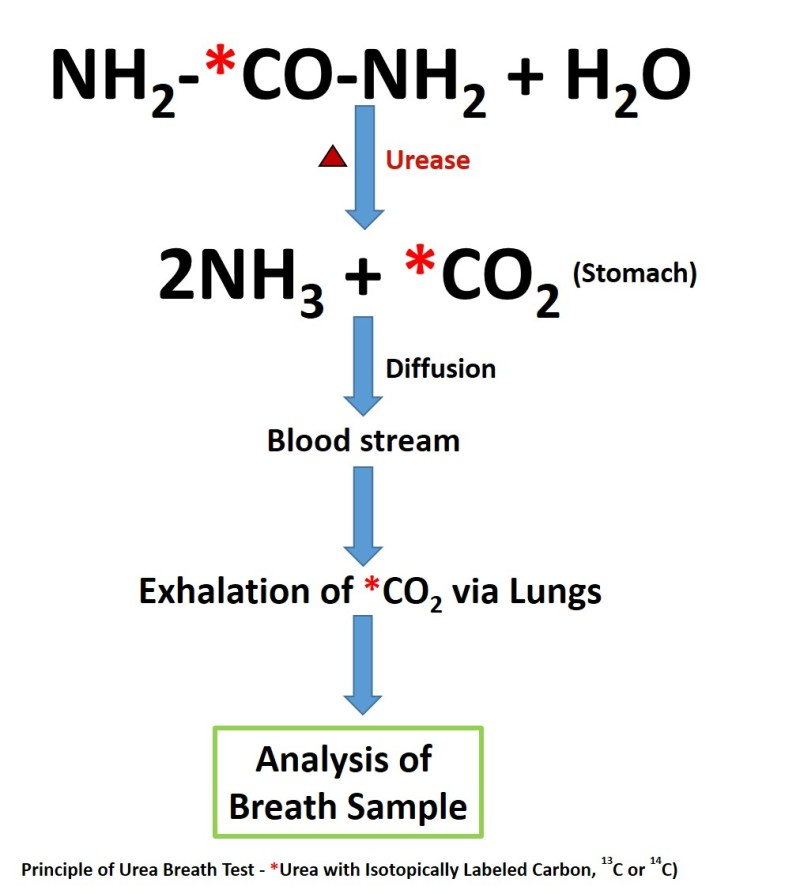
\includegraphics[width=1\linewidth]{./figure/urea_test.jpg}
    \caption{Urea breath test pathway. Borrowed from  Sankararaman S, Moosavi L. Urea Breath Test. [Updated 2024 Feb 23]. 
    In: StatPearls [Internet]. Treasure Island (FL): StatPearls Publishing; 2024 Jan-. Available 
    from: https://www.ncbi.nlm.nih.gov/books/NBK542286/}
    \label{fig:urea_test}
\end{figure}

\begin{tcolorbox}[breakable,
    title=Saliva,
    title filled=false,
    colback=blue!5!white,
    colframe=blue!75!black]
    Saliva is formed by an active process of ion secretion into the lumen of the gland, creating an osmotic gradient which 
    draws water through from the interstitial space. 
    \begin{itemize}
        \item Most ions and metabolites are transported by specific channels into saliva. 
        \item Proteins are synthesized in the glands and added mostly by a separate mechanism of storage granule release
        dependant on cyclic adenosine monophosphate (AMP) signaling:
        \begin{itemize}
            \item Saliva directly from the duct: few serum proteins.
            \item Whole mouth saliva: high amount of serum proteins derived from a serum transudate leaking around teeth 
            (via gingival crevicular fluid).
        \end{itemize}
        \item Urea concentrations  parotid saliva \> whole mouth saliva/plasma $\rightarrow$ active transport of urea into parotid 
        saliva + use by bacteria.
        \begin{itemize}
            \item Urea is the most non-protein nutrient in saliva, used by \textit{Streptococcus salivaris}, 
            \textit{Actinomyces naeslundii}, \textit{Haemophilus} by their expression of urease 
            (urea $\rightarrow$ ammonia + CO2 or urea $\rightarrow$ ammonium carbamate $\rightarrow$ Formate). Urease is not present in mammalian cells. 
            Indeed, this reaction is so reliable that it is the basis of the urea breath test for \textit{Helicobacter pylori} 
            infections of the gut ~\autoref{fig:urea_test}.
        \end{itemize}
        \item Low levels of sugars/carbohydrates in absence of food. Bacteria presumably rapidly utilize them via the 
        Embden Meyerhof Parnas (EMP) pathway ~\autoref{fig:saliva_content}.
        \begin{itemize}
            \item Carbohydrates sources from food are still detectable after 20min, but usually clear in the mouth after 
            1h. $\rightarrow$ CH not may fuel source for commensal bacteria. 
            \item Proteins as main fuel source by proteolytic degradation of salivary proteins. 
            \item The Arginine Deiminase System (ADS) hydrolyses arginine to create citrulline and ammonia; the ammonia 
            is beneficial to the host by neutralizing lactic acid in carious lesions. This pathway has become prominent 
            as some dental products now contain arginine as an additive. 
            \item CH linked to proteins (glycoproteins) can also be used by sialidases action and other glycosidases 
            (glycolytic EMP pathway = glucose $\rightarrow$ pyruvate). Here importance of bacteria cooperation in biofilms as no 
            single bacterium contains all the necessary enzymes involved in the EMP pathway. 
        \end{itemize}
        \item Nitrate
        \begin{itemize}
            \item Actively transported from the blood system by the salivary glands via the sialin transporter and delivered into the saliva. 
            \item Bacteria including Rothia and Veillonella nitrate $\rightarrow$ nitrite (+ stomach acid) $\rightarrow$ NO. 
            \item Cor(Salivary nitrate, lowered caries risk).
            \item Altered microbiome by long-term nitrate supplementation $\rightarrow$ utilization.
        \end{itemize}
        \item Lactate
        \begin{itemize}
            \item Connected to a high diversity in the mouth. Lactate consumers present in multi-species biolfilms 
            $\rightarrow$ syntrophy. 
            \item Actively secreted by saliva.
        \end{itemize}
        \item Bicarbonate
        \begin{itemize}
            \item Actively secreted by salivary mucin-secreting sublingual and minor glands.
            \item Consumers and producers such as Streptococcus anginosus and Porphyromonas gingivalis, respectively.
        \end{itemize}
        \item Limitation of other nutrients availability
        \begin{itemize}
            \item Chelation of iron by binding to iron-free lactoferrin. 
            \item Cobalamin (B12 vitamin). Not transport from serum to saliva + transcobalamin 
            (vitamin-binding proteins) $\rightarrow$ Prevents use by bacteria such as P. gingivalis. 
        \end{itemize}
    \end{itemize}
\end{tcolorbox}

\section{Site-specialist communities in the major oral habitats}

\begin{definition}[Site-specialist hypothesis]
    Each microbe in the mouth is specialized for one habitat or another, so that the microbiota at one oral site is different 
from the microbiota at other oral sites not onli in overall composition and proportions of common taxa but also in specific 
membership. Each taxon had a primary "ecological \gls{niche}" (e.g. teeth, tongue, or buccal mucosa) \cite{Welch2020}.
\end{definition}

Namely, it suggests that the most significant factor that determines the niche for a microbe is its local habitat, which 
includes its immediate neighbors. It implies that the co-evolution of microbes within the mouth has led to highly specific 
taxon-taxon interactions that results in most microbes being restricted to the habitat type in the mouth that is occupied 
by those neighbors.

Microbial communities at different sites in the mouth are organized similarly, in that they are composed predominantly of 
several dozen abundant and prevalent taxa from core genera that are represented in each of the site microbiomes. However, 
at the species level, the sites are distincts. This pattern of a common set of genera but different species from site to 
site, suggests that the different members of the microbial community are a adapted to one another and co-evolve as the 
community adapts from one oral site to the next \cite{Welch2020}. 

\section{Microbial habitats and niches at the micron scale}
In spatially organized ecosystems such as the oral microbiome, the physical proximity cell-to-cell plays an important 
role associations and steep gradients that are crucial in forming the habitat for each microbe.

\begin{definition}[Hedgehog]
    Outer shell of approximately 20-30 $\mu$m wide which is composed by aerobes and facultative anaerobes \cite{Welch2020}.
    Inside of this outer anaerobic shell lay a middle layer occupied by taxa that grow well in micro-aerobic conditions;
    filaments \textit{Corynebacterium} spp. were densely packed at its base and extended through the middle layer to the 
    outer shell. The deep core of the structure is rich in taxa that grow anaerobically. (include figure)
\end{definition}


In addition to habitat zones and gradients, tight cell-to-cell associations between disparate taxa are characteristic of 
oral biolfims and are the micron-scale manifestation of the molecular-level coadhesion interactions among taxa.

Distinct differences in microbial composition occur in different regions of disease-associated biolfilms.

A direct connection between spatial organization and biofilm pathogenecity was demonstrated by Kim et al 2020 studying 
\textit{Streptococcus mutants} in caries. They showed that early biofilms were thin, flat, and characterized by intermixing 
between \textit{S. mutants} and the non-pathogenic \textit{S. oralis}, whereas later biofilms formed a domed structure in 
which the two taxa segregated from one another. Production of glucans by \textit{S. mutants} was required for the segregation, 
as well as for the formation of the domed structure which was associated with demineralization of enamel.

The site specialist hypothesis holds that each taxon is restricted to a single category of site within the mouth and therefore 
is retricted to a limited set of partners, yet both spatial nearest-neighbor arrangements of taxa in oral biofilms, and 
the molecular interactions that underlie them, indicate that many taxa have a range of potential partners within a site. 
Corncobs are an example of fairly specific taxon-taxon interactions but with some flexibility in membership.

\begin{definition}[Corncobs]
    Structures in the dental plaque with highly stereotypical arrangements, with a central filaments surrounded by a single 
    or double layer of cocci. The participating cocci are non-specific (i.e. \textit{Streptococcus}, \textit{Porphyromonas},
    \textit{Haemophilus} genera).
    (include figure)
\end{definition}

\textit{Fusobacterium nucleatum} was widely thought to occupy a special position in the development and structure of the 
oral films, by being a central structural components of plaque and essential for plaque maduration and an increase in plaque 
diversity. However, recents studies suggest that \textit{F. nucleatum} does not constitute a physical bridge between early 
and late-colonizing dental plaque organisms \cite{Welch2020}. Instead, now it is believe to be an opportunistic colonizer 
and indicator of the maduration of the plaque to the point where anoxic niches become available (\textit{Fusobacterium} spp. 
are obligate anaerobes). In the dental plaque hedgehog structure with filaments of \textit{Corynebacterium} spp. form the structural bridge, reaching 
from the base of the structure to the tip where they form the core of the corncob structure that fringe the hedgehog.

Given the importance of syntrophy to the oral microbiome, the question arises of how syntrophy is maintained during growth 
of the biofilm. Due to the fact that a microbe grows more efficiently when it can receive resources from disparate microbes 
a few microns away, its growth will slow or cease when it gets too far from those syntrophic partners, creating clonal clusters  
during the process. Current hypothesis are growth in vertical columns and in a filamentous morphology, but exception in 
large patches have been shown for members of the genus \textit{Actinomyces}, \textit{Rothia mucilaginosa}, 
and \textit{Streptococcus salivarius}.

\section{Short and large-range factors}
Most likely the oral biofilms compositions are influence by the interaction of short and large-range factors:
\begin{itemize}
    \item Short-range: direct adhesion, micron-scale strong gradients.
    \item Large-range: Saliva flow composition and velocity.
\end{itemize}

Changes in the velocity of salivary flow result in changes in the clearence rate of substances from the surface of the 
biolfim, which presumably stregthen or attenuate the micron-scale gradients within the biolfilm.

Proctor2018 sampled buccal and lingual aspects of teeth in 30 individuals and found that the most abundant taxa were consistent 
regardless of location, but less-abudant taxa showed a gradient in abundance from front to back of the mouth, particularly 
at lingual sites. This study and another previous one from Simon-Soro et al 2013 found evidence for shifts in the proportions 
of the dental plaque microbiota on different teeth or different aspects of teeth, but the details of the finding differed.

It is possible that the question of how dental plaque communities shift across the mouth has not yielded a straightforward 
answer because a mistmatch between the sampling method and the size and spatial organization of the communities under study.
In short, DNA sequencing approaches can now tell us with great accuracy and completness what microbes are present in the samples 
we collected and homogenized, but the sampling technology for sequencing lacks the requisite spation resolution to investigate 
community structure. To address questions of how microbes are organized, how they interact, and how is the functional role of 
each microbe in the physiology of an oral biofilm at the sampled sites, we need analysis methods with a higher resolution and 
in which spatial organization remains as intact as possible.